%%%%%%%%%%%%%%%%%%%%%%%%%%%%%%%%%%%%%%%%%
% Short Sectioned Assignment
% LaTeX Template
% Version 1.0 (5/5/12)
%
% This template has been downloaded from:
% http://www.LaTeXTemplates.com
%
% Original author:
% Frits Wenneker (http://www.howtotex.com)
%
% License:
% CC BY-NC-SA 3.0 (http://creativecommons.org/licenses/by-nc-sa/3.0/)
%
%%%%%%%%%%%%%%%%%%%%%%%%%%%%%%%%%%%%%%%%%

%----------------------------------------------------------------------------------------
%	PACKAGES AND OTHER DOCUMENT CONFIGURATIONS
%----------------------------------------------------------------------------------------

\documentclass[paper=a4, fontsize=11pt]{scrartcl} % A4 paper and 11pt font size

\usepackage[T1]{fontenc} % Use 8-bit encoding that has 256 glyphs
\usepackage{fourier} % Use the Adobe Utopia font for the document - comment this line to return to the LaTeX default
\usepackage[english]{babel} % English language/hyphenation
\usepackage{amsmath,amsfonts,amsthm} % Math packages

\usepackage{lipsum} % Used for inserting dummy 'Lorem ipsum' text into the template

\usepackage{sectsty} % Allows customizing section commands
\allsectionsfont{\normalfont\scshape} % Make all sections centered, the default font and small caps
% \allsectionsfont{\centering \normalfont\scshape} % Make all sections centered, the default font and small caps

\usepackage{fancyhdr} % Custom headers and footers
\usepackage{graphicx}
\pagestyle{fancyplain} % Makes all pages in the document conform to the custom headers and footers
\fancyhead{} % No page header - if you want one, create it in the same way as the footers below
\fancyfoot[L]{} % Empty left footer
\fancyfoot[C]{} % Empty center footer
\fancyfoot[R]{\thepage} % Page numbering for right footer
\renewcommand{\headrulewidth}{0pt} % Remove header underlines
\renewcommand{\footrulewidth}{0pt} % Remove footer underlines
\setlength{\headheight}{13.6pt} % Customize the height of the header

\numberwithin{equation}{section} % Number equations within sections (i.e. 1.1, 1.2, 2.1, 2.2 instead of 1, 2, 3, 4)
\numberwithin{figure}{section} % Number figures within sections (i.e. 1.1, 1.2, 2.1, 2.2 instead of 1, 2, 3, 4)
\numberwithin{table}{section} % Number tables within sections (i.e. 1.1, 1.2, 2.1, 2.2 instead of 1, 2, 3, 4)

\setlength\parindent{0pt} % Removes all indentation from paragraphs - comment this line for an assignment with lots of text

%----------------------------------------------------------------------------------------
%	TITLE SECTION
%----------------------------------------------------------------------------------------

\newcommand{\horrule}[1]{\rule{\linewidth}{#1}} % Create horizontal rule command with 1 argument of height

\title{	
\normalfont \normalsize 
\textsc{CSIT 6000F} \\ [25pt] % Your university, school and/or department name(s)
\horrule{0.5pt} \\[0.4cm] % Thin top horizontal rule
\huge Assignment 1 \\ % The assignment title
\horrule{2pt} \\[0.5cm] % Thick bottom horizontal rule
}

\author{Yuchen, GUO} % Your name

\date{\normalsize\today} % Today's date or a custom date

\begin{document}

\maketitle % Print the title

%----------------------------------------------------------------------------------------
%	PROBLEM 1
%----------------------------------------------------------------------------------------

\section{Problem 1}

In this problems, we can describe the input of the sensors using a matrix:

\begin{align*}
S = 
\begin{bmatrix}
    s_1 & s_2 & s_3\\
    s_8 & - & s_4\\
    s_7 & s_6 & s_5
\end{bmatrix}
\end{align*}

So the ball has only 9 exclusive states as following:

\begin{align*}
S_1 = 
\begin{bmatrix}
    1 & 1 & 1\\
    1 & - & 0\\
    1 & 0 & 0
\end{bmatrix},
S_2 = 
\begin{bmatrix}
    1 & 1 & 1\\
    0 & - & 0\\
    0 & 0 & 0
\end{bmatrix},
S_3 = 
\begin{bmatrix}
    1 & 1 & 1\\
    0 & - & 1\\
    0 & 0 & 1
\end{bmatrix},\\
S_4 = 
\begin{bmatrix}
    1 & 0 & 0\\
    1 & - & 0\\
    1 & 0 & 0
\end{bmatrix},
S_5 = 
\begin{bmatrix}
    0 & 0 & 0\\
    0 & - & 0\\
    0 & 0 & 0
\end{bmatrix},
S_6 = 
\begin{bmatrix}
    0 & 0 & 1\\
    0 & - & 1\\
    0 & 0 & 1
\end{bmatrix},\\
S_7 = 
\begin{bmatrix}
    1 & 0 & 0\\
    1 & - & 0\\
    1 & 1 & 1
\end{bmatrix},
S_8 = 
\begin{bmatrix}
    0 & 0 & 0\\
    0 & - & 0\\
    1 & 1 & 1
\end{bmatrix},
S_9 = 
\begin{bmatrix}
    0 & 0 & 1\\
    0 & - & 1\\
    1 & 1 & 1
\end{bmatrix},
\end{align*}

Below are the original form of $S_1$ to $S_9$:

\begin{align*}
S_1 = s_1 \cdot s_2 \cdot s_3 \cdot \overline{s_4} \cdot \overline{s_5} \cdot \overline{s_6} \cdot s_7 \cdot s_8\\
S_2 = s_1 \cdot s_2 \cdot s_3 \cdot \overline{s_4} \cdot \overline{s_5} \cdot \overline{s_6} \cdot \overline{s_7} \cdot \overline{s_8}\\
S_3 = s_1 \cdot s_2 \cdot s_3 \cdot s_4 \cdot s_5 \cdot \overline{s_6} \cdot \overline{s_7} \cdot \overline{s_8}\\
S_4 = s_1 \cdot \overline{s_2} \cdot \overline{s_3} \cdot \overline{s_4} \cdot \overline{s_5} \cdot \overline{s_6} \cdot s_7 \cdot s_8\\
S_5 = \overline{s_1} \cdot \overline{s_2} \cdot \overline{s_3} \cdot \overline{s_4} \cdot \overline{s_5} \cdot \overline{s_6} \cdot \overline{s_7} \cdot \overline{s_8}\\
S_6 = \overline{s_1} \cdot \overline{s_2} \cdot s_3 \cdot s_4 \cdot s_5 \cdot \overline{s_6} \cdot \overline{s_7} \cdot \overline{s_8}\\
S_7 = s_1 \cdot \overline{s_2} \cdot \overline{s_3} \cdot \overline{s_4} \cdot s_5 \cdot s_6 \cdot s_7 \cdot s_8\\
S_8 = \overline{s_1} \cdot \overline{s_2} \cdot \overline{s_3} \cdot \overline{s_4} \cdot s_5 \cdot s_6 \cdot s_7 \cdot \overline{s_8}\\
S_9 = \overline{s_1} \cdot \overline{s_2} \cdot s_3 \cdot s_4 \cdot s_5 \cdot s_6 \cdot s_7 \cdot \overline{s_8}\\
\end{align*}

%------------------------------------------------

\subsection{}

Let's take the northwest corner for example.\\

When the ball is not next to the north border, move it to north, otherwise move it to west\\

Here is the production system:\\

\boldmath \begin{align*}
&\overline{s_2} \longrightarrow north\\
&\overline{s_8} \longrightarrow west
\end{align*}
or
\boldmath \begin{align*}
&S_2+S_3 \longrightarrow west\\
&S_4+S_5+S_6+S_7+S_8+S_9 \longrightarrow north
\end{align*}

%------------------------------------------------

\subsection{}

We can put the robot in the center of the grid, and prove it can't visit every cell.

With $S_5$, it can move in any direction in ${north, west, east, south}$, in the following figure, 
we assume it be west, and it can be any direction by rotating the image, 
the situations are equivalent.

The robot with move in the same direction until it reaches a border.
Then let's see how can its state transfer to $S_5$ again,
all possible ways are marked with pointers in the left part of Figure ~\ref{fig:Problem1.2.1}, 
the right part shows possible circles that the robot can move in(equivalent paths are ignored).\\
    
\begin{figure}[p]
    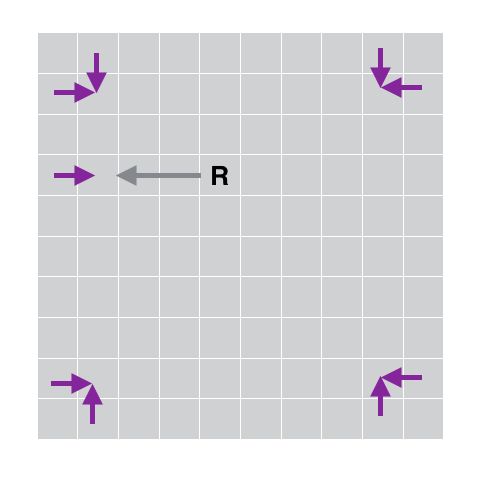
\includegraphics[scale=0.5]{image1.png}
    \hspace{\fill}
    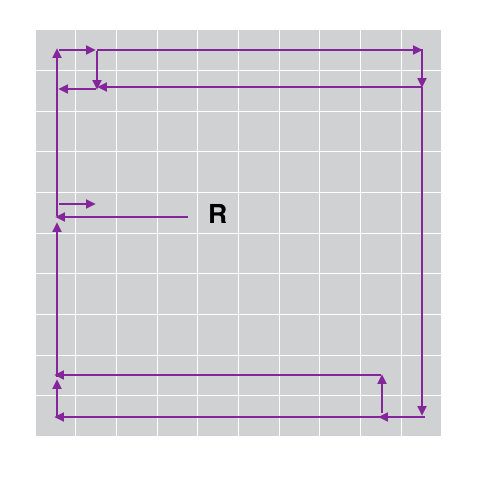
\includegraphics[scale=0.5]{image2.png}
    \caption{Ways to enter $S_5$ again and possible circles}
    \label{fig:Problem1.2.1}
    \vspace{\fill}
    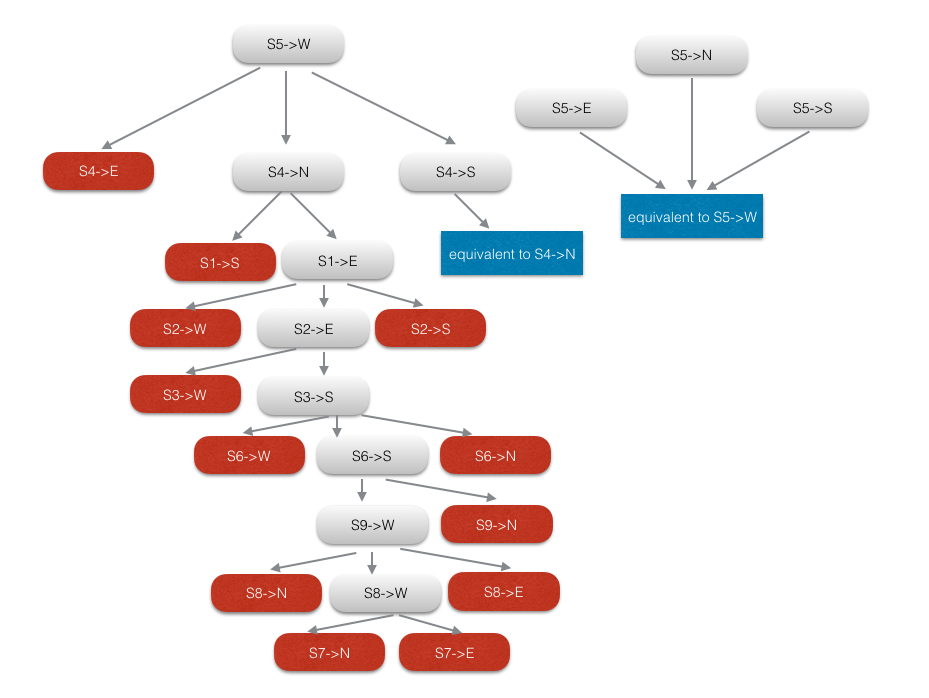
\includegraphics[scale=0.5]{image6.png}
    \caption{Search tree to find production system that can visit all cells, 
        red nodes means the robot is going to move in a circle of several nodes,
        blue nodes means the situation is equivalent to another one, as we can see,
        all paths ends with a red node.}
    \label{fig:Problem1.2.2}
\end{figure}

Figure ~\ref{fig:Problem1.2.2} shows all production systems makes the robot move between 
some cells(Not all cells in the grid).
So in no way can the robot visit cells far from the border. 
Thus it's not possible to visit every cell in the grid.\\

%------------------------------------------------
\subsection{Part 3 of Problem 1}

Let $W_{ij}$ be the features defined as:\\
$W_{ij}$ = 1 iff at the previous time step, $S_i$ = 1, and the robot moved $j$($j$ is in ${N, W, E, S}$).
For example:
$W_{1E}$ = 1 iff at the previous time step, $S_1$ = 1, and the robot moved $East$.\\

\begin{figure}[h]
    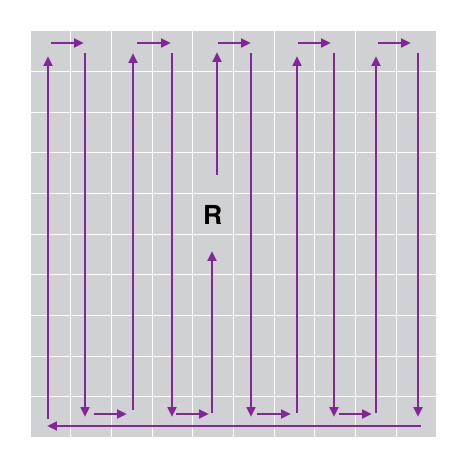
\includegraphics[scale=0.5]{image3.png}
    \hspace{\fill}
    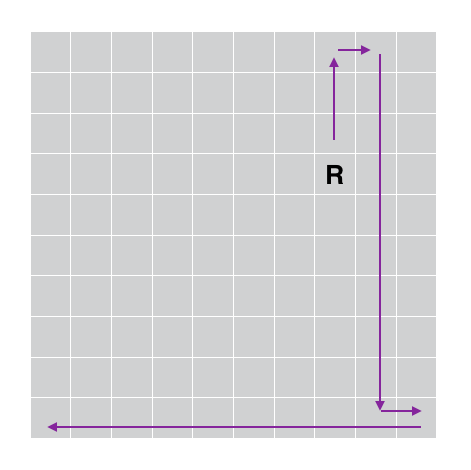
\includegraphics[scale=0.5]{image4.png}
    \caption{Two situations to visit all cells}
    \label{fig:Problem1.3}
\end{figure}

As Figure ~\ref{fig:Problem1.3} shows, we want the robot to visit every cell 
in the route in the left picutre.

Here is the production system:
\boldmath \begin{align*}
&S_2 \cdot W_{5N} \longrightarrow east\\
&S_2 \cdot (W_{2E} + W_{1E}) \longrightarrow south\\
&S_5 \cdot (W_{2S}+W_{5S}) \longrightarrow south\\
&S_5 \cdot (W_{8N}+W_{5N}) \longrightarrow north\\
&S_8 \cdot W_{5S} \longrightarrow east\\
&S_8 \cdot W_{8E} \longrightarrow north\\
&S_8 \cdot (W_{8W}+W_{9W}) \longrightarrow west\\
&S_1 \longrightarrow east\\
&S_3+S_6 \longrightarrow south\\
&S_4+S_5+S_7 \longrightarrow north\\
&S_9 \longrightarrow west\\
&1 \longrightarrow north
\end{align*}

%----------------------------------------------------------------------------------------
%	PROBLEM 2
%----------------------------------------------------------------------------------------

\section{Problem 2}

Let the input be $A, B, C, D, E$. Then:

\begin{align*}
Result=(1.1*A+3.1*B-C-2*D+0.5*E>1)\\
\end{align*}

Accoding to the inequation above:\\
If $C \cdot D$, $Result=1$ iff $1.1*A+3.1*B+0.5*E>4$ iff $A \cdot B$\\
If $C \cdot \overline{D}$, $Result=1$ iff $1.1*A+3.1*B+0.5*E>2$ iff $B$\\
If $\overline{C} \cdot D$, $Result=1$ iff $1.1*A+3.1*B+0.5*E>3$  iff $B$\\
If $\overline{C} \cdot \overline{D}$, $Result=1$ iff $1.1*A+3.1*B+0.5*E>1$ iff $A + B$\\

So:

\begin{align*}
Result&= C \cdot D \cdot A \cdot B + 
         C \cdot \overline{D} \cdot B +
         \overline{C} \cdot D \cdot B +
         \overline{C} \cdot \overline{D} \cdot (A + B)\\
      &= A \cdot B \cdot C \cdot D + 
         A \cdot \overline{C} \cdot \overline{D} +
         B \cdot (\overline{C} \cdot \overline{D} + C \cdot \overline{D} + \overline{C} \cdot D)\\
      &= A \cdot B \cdot C \cdot D + 
         (A + 1) \cdot B \cdot (\overline{C} \cdot \overline{D} + C \cdot \overline{D} + \overline{C} \cdot D) +
         A \cdot \overline{C} \cdot \overline{D}\\
      &= A \cdot B \cdot C \cdot D + 
         A \cdot B \cdot (\overline{C} \cdot \overline{D} + C \cdot \overline{D} + \overline{C} \cdot D) +
         B \cdot (\overline{C} \cdot \overline{D} + C \cdot \overline{D} + \overline{C} \cdot D) +
        %  B \cdot (\overline{C} + \overline{D}) +
         A \cdot \overline{C} \cdot \overline{D} \\
      &= A \cdot B \cdot (C \cdot D + \overline{C} \cdot \overline{D} + C \cdot \overline{D} + \overline{C} \cdot D) +
         A \cdot \overline{C} \cdot \overline{D} +
         B \cdot (\overline{C} + \overline{D})\\
      &= A \cdot B +
         A \cdot \overline{C} \cdot \overline{D} +
         B \cdot (\overline{C} + \overline{D}) 
\end{align*}

%----------------------------------------------------------------------------------------

%----------------------------------------------------------------------------------------
%	PROBLEM 3
%----------------------------------------------------------------------------------------

\section{Problem 3}

Here is the breadth-first search process:

\begin{figure}[h]
    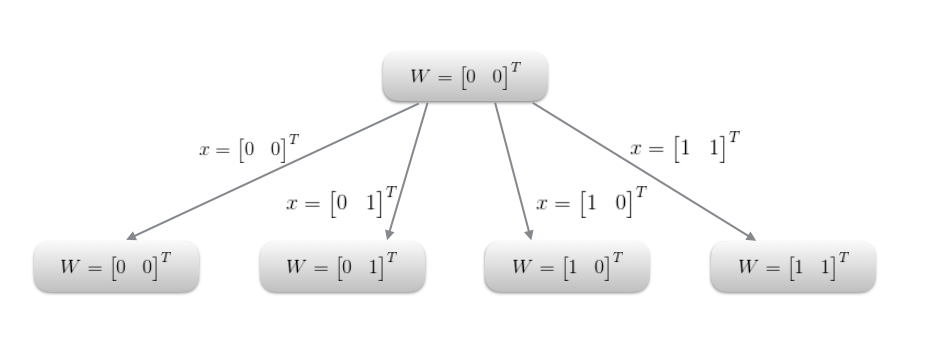
\includegraphics[scale=0.5]{image5.png}
    \caption{Breadth-first search to do error-correction}
    \label{fig:Problem3.1}
\end{figure}

%----------------------------------------------------------------------------------------

%----------------------------------------------------------------------------------------
%	PROBLEM 4
%----------------------------------------------------------------------------------------

\section{Problem 4}

\subsection{}

Total floors the elevator moved when it transfered the last people.

\subsection{}

Total time all vehicles and passerbys waited at the crossroad.

%----------------------------------------------------------------------------------------

%----------------------------------------------------------------------------------------
%	PROBLEM 5
%----------------------------------------------------------------------------------------

\section{Problem 5}

Feature:\\
$F_1$: cricket is on the threshold\\
$F_2$: all is well in the burrow\\

Action:\\
$A_1$: move the cricket to the threshold\\
$A_2$: check inside\\
$A_2$: go outside to the threshold\\
$A_3$: drag the cricket inside\\

Production System:\\
\begin{align*}
\overline{F_1} \longrightarrow A_1\\
F_1 \longrightarrow A_2\\
\end{align*}



%----------------------------------------------------------------------------------------
\end{document}